\documentclass[english]{ijsra}
\def\IJSRAidentifier{\currfilebase}%<<<< DO NOT change this line

%-------Title | Email | Keywords | Abstract-------------
\def\shorttitle{AAPA 2016 Review}
\def\maintitle{Review: American Association of Physical Anthropologists 2016 Annual Meeting}
\def\cmail{}
\def\keywords{Review, Annual Meeting, 85th}
%\def\keywordname{}
%\undef\abstract

%--------Author’s names------------
\def\authorone{Devin L. Ward}
\def\authortwo{Michael B. C. Rivera}
\def\authorthree{Jaap P. P. Saers}

%-------Biographical information-------------
\def\bioone{Devin L. Ward (https://utoronto.academia.edu/DevinWard) is a first year PhD Student at the University of Toronto and a Junior Fellow at Massey College, where she studies shape variation in the human inner ear.
At the 2016 AAPA meeting, she presented research conducted for completion of her MPhil in Biological Anthropological Science at the University of Cambridge titled, “\emph{Insights into Developmental Stress Exposure from the Bony Labyrinth}”.
Devin is also an Editor of the International Journal of Student Research in Archaeology and is involved in ongoing bioarchaeological projects in Gibraltar and Italy.}
\def\biotwo{Michael B. C. Rivera (https://cambridge.academia.edu/MichaelRivera) is a PhD student at the University of Cambridge conducting research on bioarchaeology and coastal adaptations in the prehistoric Baltics (between 5,400\BC–450\AD).
His other interests include global human skeletal variation—at the 2016 AAPA meeting, he presented a poster on climatic adaptation and neutral evolution of the human lower limb.
Michael is a Reviewer for the International Journal of Student Research in Archaeology and a co-organizer of the 4th Annual Student Archaeology Conference (the proceedings of which will be published in the next issue of the IJSRA).}
\def\biothree{Jaap P. P. Saers (https://cambridge.academia.edu/JaapSaers) is a PhD candidate at Cambridge University.
His research focuses on the interaction between growth and development, physical activity, and the structural organization of human trabecular bone.}%add hyperlinks to above?

%------University/Institution--------------
\def\affilone{Department of Anthropology, University of Toronto}
\def\affiltwo{Department of Archaeology \& Anthropology, University of Cambridge}

%--------Mapping of authors to affiliations------------
%% authorone:--> * <--- copy/paste that symbol to \affiloneauthor etc. below
%% authortwo:--> † <--- copy/paste that symbol to \affiloneauthor etc. below
%% authorthree:--> ‡ <--- copy/paste that symbol to \affiloneauthor etc. below
%% authorfour: --> § <--- copy/paste that symbol to \affiloneauthor etc. below
%% authorfive: --> ¶ <--- copy/paste that symbol to \affiloneauthor etc. below
%-------------------------------------------------------------------------
\def\affiloneauthor{*}%<---- paste the symbol of the authors into {}
\def\affiltwoauthor{†}%<---- paste the symbol of the authors into {}
\def\affilthreeauthor{†}%<---- paste the symbol of the authors into {}

\begin{filecontents}{\IJSRAidentifier.bib}
@misc{beasley_2016,
title = {A Guide to Student Events at the 2016 AAPA Annual Meeting},
url = {http://physanth.org/news/738/},
journal = {American Association of Physical Anthropologists},
publisher = {American Association of Physical Anthropologists},
author = {Beasley, Melanie},
year = {2016},
month = {Mar}
} 

@misc{american association of physical anthropologists_2015,
title = {Committee on Diversity Women's Initiative Graduate Student Women's Professional Development Workshop},
url = {http://physanth.org/news/654/},
journal = {American Association of Physical Anthropologists},
publisher = {American Association of Physical Anthropologists},
year = {2015},
month = {Dec}
}

@misc{american association of physical anthropologists,
title = {Student presentation awards},
url = {http://physanth.org/about/awards/student-presentation-awards},
journal = {American Association of Physical Anthropologists},
publisher = {American Association of Physical Anthropologists}
}

@misc{american association of physical anthropologists_2016,
title = {American Association of Physical Anthropologists},
url = {http://www.physanth.org/},
journal = {American Association of Physical Anthropologists},
publisher = {American Association of Physical Anthropologists},
year = {2016}
}
\end{filecontents}

\begin{document}
\IJSRAopening%<<<< DO NOT change this line


\lettrine{T}he \IJSRAsection{Introduction} 85th annual meeting of the American Association of Physical Anthropologists (AAPA)
took place April 13‒17, in Atlanta, Georgia, USA (\cref{fig:Ward-Figure1},,{fig:Ward-Figure2}).
Founded in 1930 with only 83 members, the Association currently has more than 1,700 members internationally \parencite{american association of physical anthropologists_2016}.
This year’s host institutions were Georgia State University and Georgia Perimeter College,
but related lectures were also held at nearby Emory University.
The AAPA invites members from all academic career stages, and annual meetings provide many opportunities to
specifically foster student involvement in physical anthropology.
Students participate in all aspects of the meetings, from presenting research through poster and
podium presentations to organization of the event itself \parencite{beasley_2016}.
Although the AAPA was well-attended by many non-student anthropologists, this review will focus on the roles of,
and opportunities for, students.

\begin{figure} %Figure 1
		\includegraphics[width=\linewidth]{figures/Ward-Figure1}
		\caption{The many levels of the conference venue, the Atlanta Marriott Marquis, leading a few delegates to liken its appearance to a spinal column and rib cage! (Copyright to authors).}
		\centering
		\label{fig:Ward-Figure1}
	\end{figure}

\begin{figure} %Figure 2
		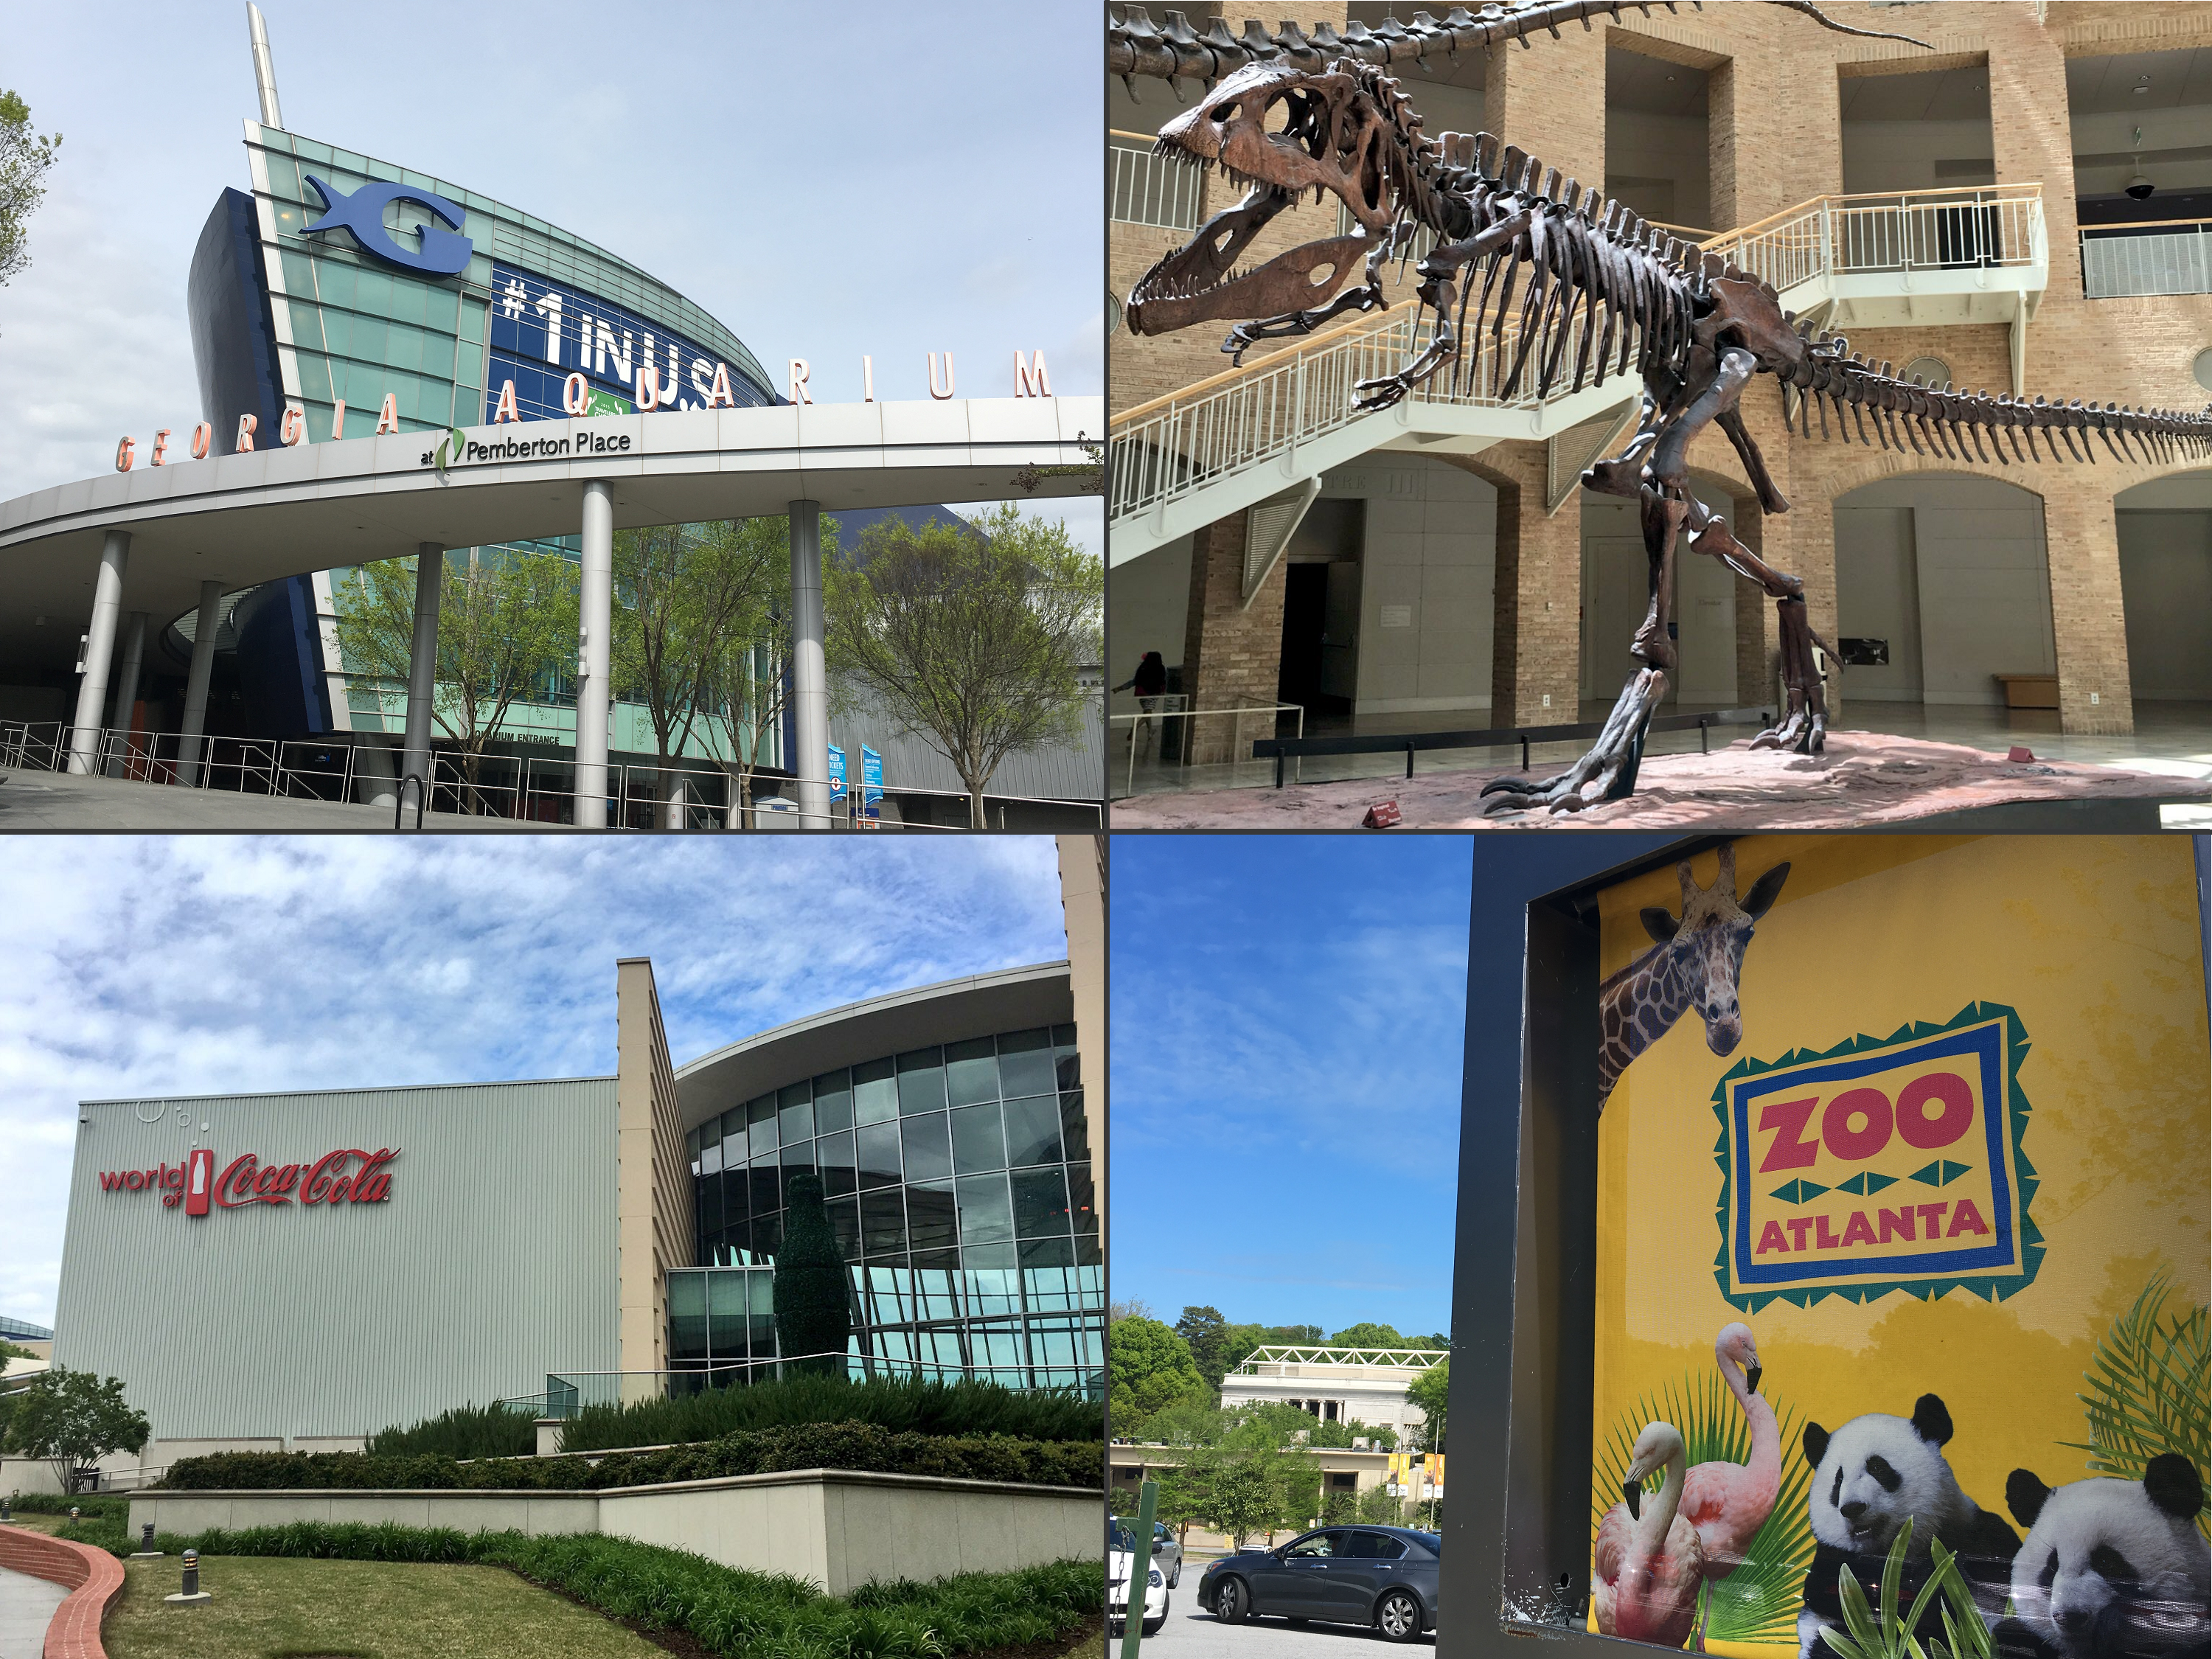
\includegraphics[width=\linewidth]{figures/Ward-Figure2}
		\caption{Attractions to enjoy in Atlanta between conference sessions included the Georgia Aquarium, the Fernbank Museum of Natural History, The World of Coca-Cola and Atlanta Zoo (Copyright to authors).}
		\centering
		\label{fig:Ward-Figure2}
	\end{figure}

The 2016 program ran over three full days and included 1,096 scientific presentations divided into 58 sessions.
These then were divided into morning and afternoon sessions, 
with approximately 4‒7 sessions being conducted concurrently per morning/afternoon. 
Many of the symposia were open to students to submit abstracts for in mid-September 2015.
Most poster and podium sessions were open to contributions from all members of the AAPA, including students,
and focused on broad topics within biological anthropology.
Topics included functional morphology, bioarcheology, primate behavior, growth and development, human genetic variation,
among others (\crefs{fig:Ward-Figure3},,{fig:Ward-Figure4}).
Poster sessions lasted all day, leaving time for attendants to browse during breaks.
The authors of each poster stood by their posters for questions as well during two designated half-hour intervals on
the day of their session (\crefs{fig:Ward-Figure5},,{fig:Ward-Figure6}).

\begin{figure} %Figure 3
		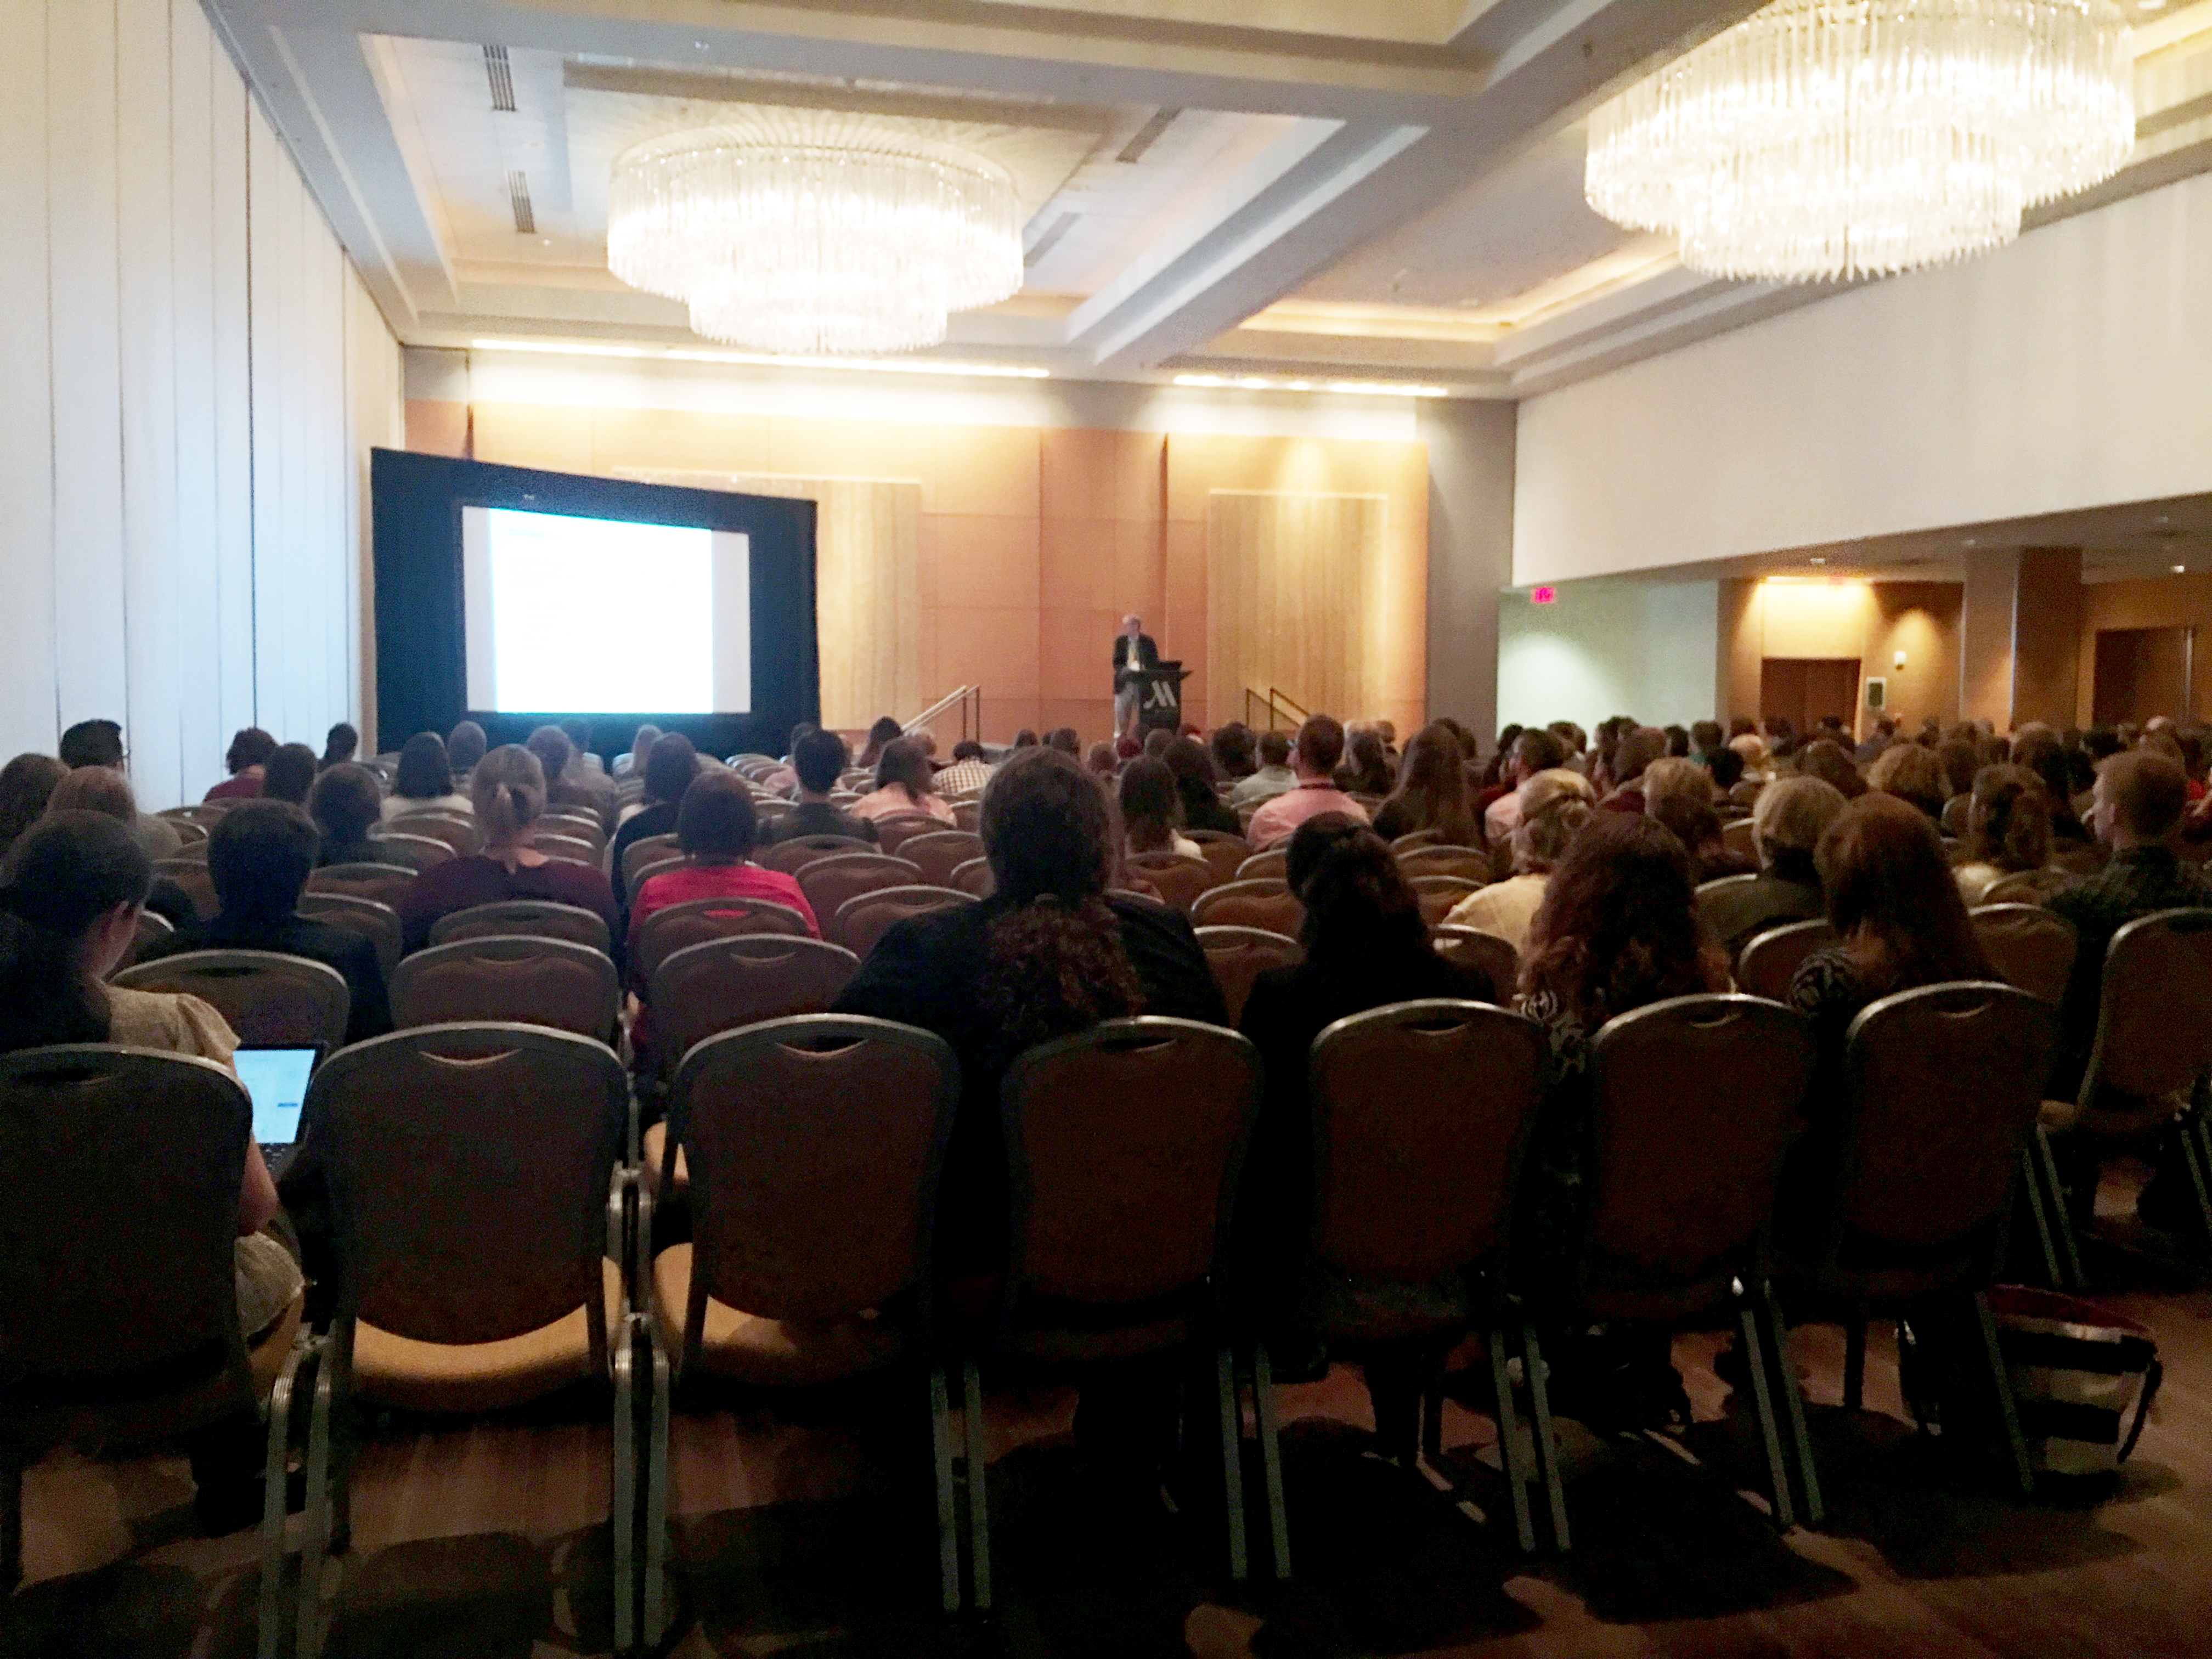
\includegraphics[width=\linewidth]{figures/Ward-Figure3}
		\caption{Podium presentations were given by undergraduates, postgraduates, post-doctoral researchers and senior faculty (Copyright to authors).}
		\centering
		\label{fig:Ward-Figure3}
	\end{figure}
	
	\begin{figure} %Figure 4
		\includegraphics[width=\linewidth]{figures/Ward-Figure4}
		\caption{The ‘Evolutionary Perspectives to Bioarchaeology’ poster symposium, hosted by Dr. Jim Watson—one of the concurrent sessions that took place in the afternoon on Thursday April 21st (Copyright to authors).}
		\centering
		\label{fig:Ward-Figure4}
	\end{figure}
	
	\begin{figure} %Figure 5
		\includegraphics[width=\linewidth]{figures/Ward-Figure5}
		\caption{Student research posters were displayed everyday in the Marriott's Atrium Ballroom (Copyright to authors).}
		\centering
		\label{fig:Ward-Figure5}
	\end{figure}
	
	\begin{figure} %Figure 6
		\includegraphics[width=\linewidth]{figures/Ward-Figure6}
		\caption{University of Cambridge PhD student Jaap Saers presenting his poster on trabecular bone morphology as part of the session, '\emph{Bone Microstructure: Imaging, Analysis and Function}' (Copyright to authors).}
		\centering
		\label{fig:Ward-Figure6}
	\end{figure}

In addition to these broad sessions, 
invited poster and podium sessions allowed dedicated idea exchanges within specialized research areas. 
There were 7 invited podium sessions and 16 invited poster symposiums covering topics such as: humans in marginal environments, 
malaria in antiquity, the morphology of the last common ancestor, and imaging and analysis of bone microstructure, to name a few. 
Invited poster symposia included a brief talk by each invited author, followed by conversation and questions. 
Each invited poster session concluded with a discussion featuring one or several prominent members of the relevant field,
where findings of the symposium were summarized and debated. 
Invited podium sessions followed a similar format where each session would be concluded by one or several discussants who synthesized
the work at the end and directed a subsequent discussion. 
Several invited podium sessions discouraged questions after each talk in order to have a more detailed discussion at the end.
One of the most popular invited podium sessions was devoted to addressing the most recent addition to the hominin fossil record,
\emph{Homo naledi}, providing the opportunity for 13 members of the Rising Stars team (mostly early-career scientists)
to present their ongoing work. 
This then culminated with a special luncheon and lecture hosted by renowned paleoanthropologist Lee Berger (\cref{fig:Ward-Figure7}).

	\begin{figure} %Figure 7
		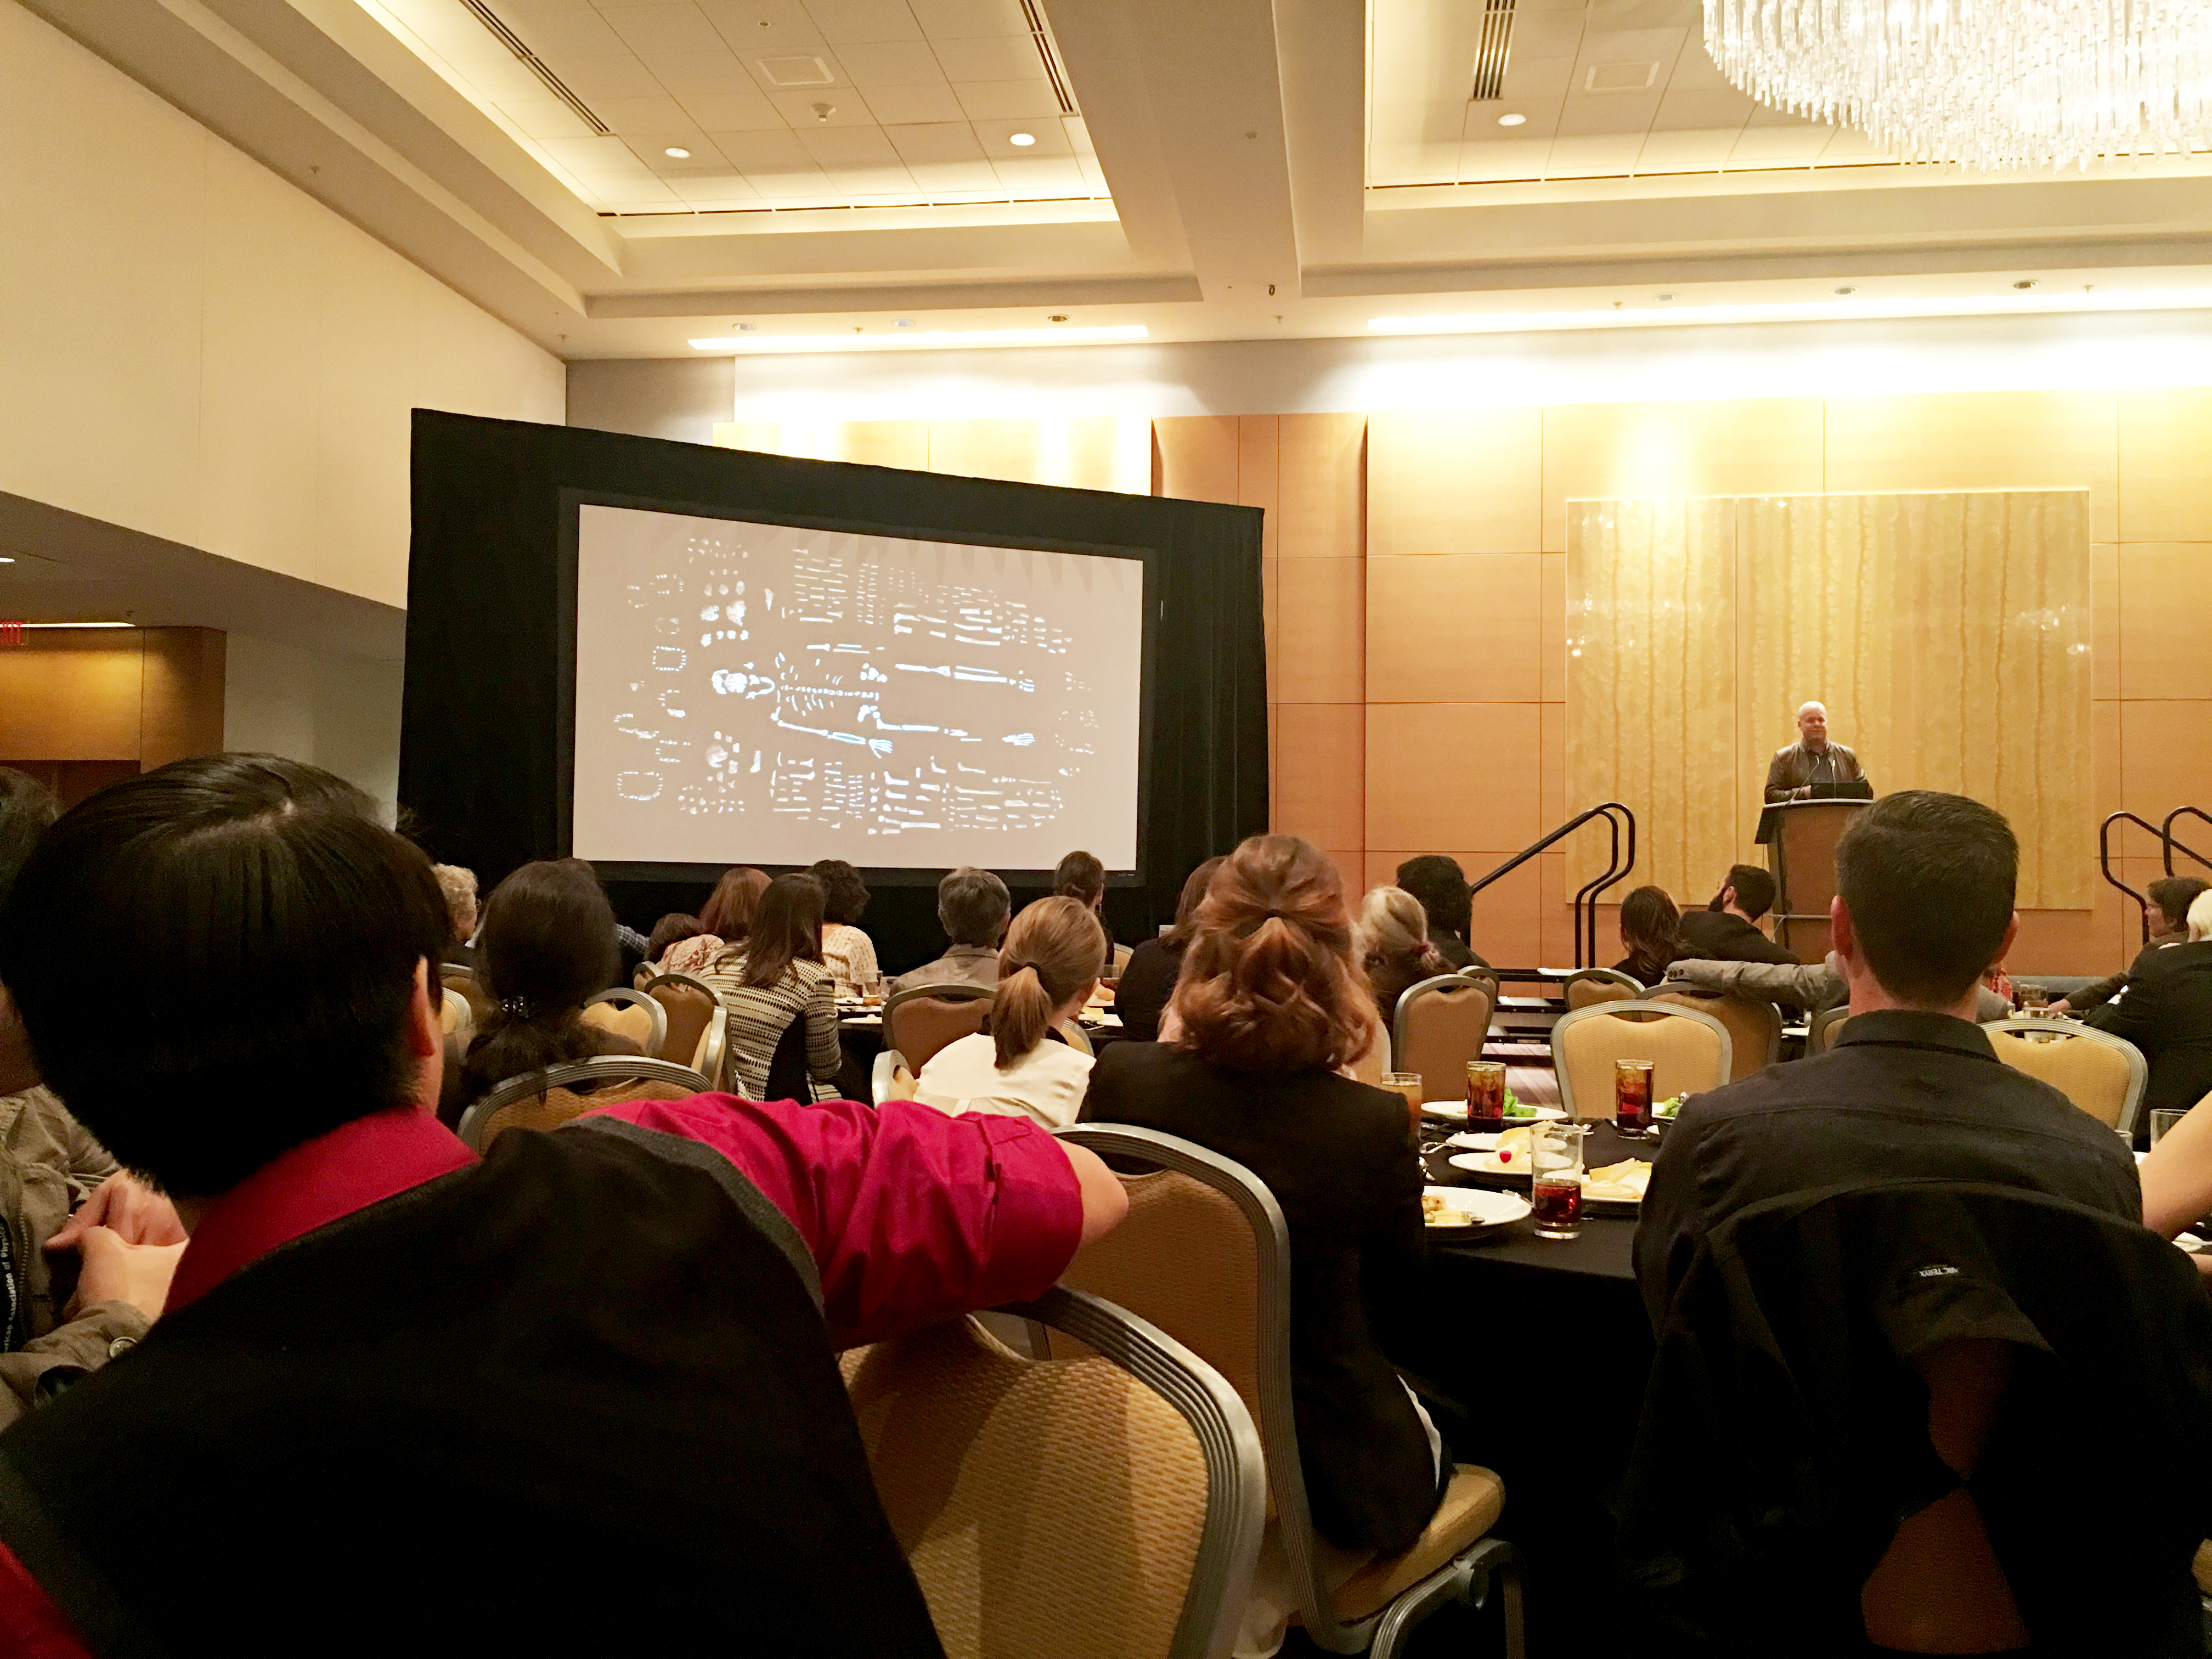
\includegraphics[width=\linewidth]{figures/Ward-Figure7}
		\caption{Lee Berger gives a luncheon presentation on the new \emph{Homo naledi} discovery, to which many students attended (Copyright to authors).}
		\centering
		\label{fig:Ward-Figure7}
	\end{figure}

Complementing these talks and poster sessions over the course of the meeting were a number of smaller panel discussions,
workshops, adjacent committee meetings, and evening receptions. 
A student awards ceremony and closing reception was the final event of this year’s event.  
All of these will be discussed in more detail throughout this review.

Graduate \IJSRAsection{Student Research} and undergraduate research is scattered throughout the meetings as posters or presentations
from faculty of all career stages within the particular session its topic fits best. Undergraduate students are additionally invited
to participate in the Undergraduate Research Symposium (URS) (\cref{fig:Ward-Figure8}), organized by Dr. Cara Wall-Scheffler
(Seattle Pacific University) and the Committee on Diversity.  
Similar to submitting for the AAPA meetings, students complete an online application.
However, the range of topics accepted for the URS is more extensive than those accepted for the overall meeting.
Undergraduate student participants are mentored by graduate student members of AAPA,
who are invited to participate as mentors on a yearly basis.
Many previous URS participants opt to continue as graduate mentors once they enter a graduate program.

	\begin{figure} %Figure 8
		\includegraphics[width=\linewidth]{figures/Ward-Figure8}
		\caption{Dr. Susan Antón gives out prizes to the participants of the Undergraduate Research Symposium (Copyright to authors).}
		\centering
		\label{fig:Ward-Figure8}
	\end{figure}

As previously mentioned, there are multiple student prizes awarded every year in many fields,
recognizing both diverse and excellent student work in the form of posters and podium presentations. 
Several of these prizes are sponsored by the AAPA in cooperation with other societies,
such as the American Association of Anatomists (AAA). 
Other prizes are in honor of specific anthropologists, including the Aleš Hrdlička Prize,
named after the founder of the American Journal of Physical Anthropology \parencite{american association of physical anthropologists}.
All of the 2016 winners were graduate students from American and Canadian universities. 
Honorable mentions went to Melanie Beasley, Amanda Lee, Brittany, and Lu Yao.  
Winners are listed as follows: 
\begin{description}
  \item[$\bullet$] Eric Castillo (Harvard University): AAA-AAPA Podium Prize for his presentation titled, “\emph{Testing biomechanical models for lumbar lordosis variation in hominins}”.
  \item[$\bullet$] Jesse Goliath (Ohio State University): AAA-AAPA Poster Prize for his poster titled, “\emph{Patterns in ontogeny of epiphyseal and metaphyseal trabecular bone microstructure in the human proximal tibia}".
  \item[$\bullet$] Andrew Halley (University of California, Berkeley): Aleš Hrdlička Prize for his podium presentation titled “\emph{The embryonic origins of primate encephalization: allometric and growth analyses}”.
  \item[$\bullet$] Myra Laird (New York University): Earnest Hooton Best Poster Prize for her poster titled, “\emph{Gape cycle kinematic variance and occlusal topography in modern humans}”.
  \item[$\bullet$] Cecilia Mayer (Macalester College): Sherwood Washburn Prize for her poster presentation titled “\emph{How tough is the grey-cheeked mangabey? Patterns of healed skeletal trauma in \emph{Lophocebus albigena}}”.
  \item[$\bullet$] Nathan Thompson (Stony Brook University): Mildred Trotter Prize for his presentation titled “\emph{In search of the last common ancestor: perspectives on the ancestral morphotype of hominins}”.
  \item[$\bullet$] Amber Walker-Bolton (University of Toronto): Juan Comas Prize for her podium presentation titled “\emph{Operational sex ratio, dominance rank and mating success of group and non-group male ring-tailed lemurs (\emph{Lemur catta})}”.
\end{description}

There \IJSRAsection{Other Student Involvement} are many ways in which students can be involved in the AAPA meetings beyond research presentation.  These opportunities have included more traditional positions, such as membership on the student committee, but in recent years the larger role of social media in conferences has opened many other doors.  

All sessions, both podium and presentation, as well as many seminars were live-tweeted.
A call for volunteer live-tweeters was put out via Twitter and departmental mailing lists by Austin Reynolds,
a University of Texas at Austin graduate student. 
The team assembled for this task comprised undergraduates, graduates, and post-doctoral researchers, 
who live-tweeted sessions covering subjects of their own research. 
Using the \#AAPA2016 hashtag, all tweets associated with this year’s meeting were easy to locate on Twitter. 
Volunteers also designed additional hashtags unique to each podium and poster session to allow Twitter users to
follow conversations of interest to them (e.g., \#ancientalleles, \#EvoBioArch, \#SEBioArch, \emph{etc.}).%add links for #ancientalleles, #EvoBioArch, #SEBioArch ?

Because many of the sessions ran parallel to each other, the use of Twitter enabled AAPA attendees to ‘listen in’ on multiple sessions simultaneously. 
Overall, live-tweeting created many positive interactions and lively discussions between early-career scientists and senior faculty members alike, both in Atlanta and among other interested academics around the world.
Unsurprisingly, many delegates attending this year’s meeting commented positively on the use of social media, as the initiative has been successful at previous meetings in recent years.

The \IJSRAsection{Networking} AAPA strives every year to provide multiple opportunities at meetings for student networking.
This year, for example, immediately following the Student Committee meeting, 
the Student Liaison and Early Career AAPA Representatives group hosted a “Meet and Greet” open to all students,
but particularly aimed towards first-time attendees. 
Before the meeting began, organizers created a Facebook group for the event and posted biographies of several “Early Career Mentors”,
early career anthropologists, who were recruited to attend the event.
This allowed students to prepare questions regarding careers and graduate school for specific mentors in advance.  
Mentors available for discussion and questions included Dr. Amy Bauernfeind (Washington University),
Dr. Chris Schmitt (Boston University), Dr. Amy Lu (Stony Brook University), Dr. Jon Bethard (Boston University),
Dr. Ashley Hammond (George-Washington University), Dr. Marissa Macias (American Museum of Natural History),
Dr. Nikki Burt (Cleveland Museum of Natural History), Dr. Christine Lee (California State University, Los Angeles),
and Dr. Scott Maddux (University of Missouri).
This event aimed to connect students of all educational stages and early career members of the AAPA from multiple subfields.  

This year, the AAPA also offered non-traditional types of networking opportunities to students,
such as the opportunity for students to interact with well-known, anthropology “luminaries”. 
Students entered one of six “Lunches with Luminaries” drawings for the chance to win a free lunch with two senior anthropologists. 
Corinna Most (graduate student at UC San Diego), Marie Vergamini (graduate student at Virginia Commonwealth University),
Lydia Light (graduate student at University of Texas, San Antonio),
and Diego Hernandez (graduate student Virginia Commonwealth University) won lunch with Dr. John Nitani and Dr. Karen Strier. 
Yajaira Gonzalez (graduate student at UC San Diego), Mary Studebaker-Reed (graduate student at Boston University School of Medicine),
David Hansen (graduate student at Central Michigan University), 
and Kelly Blevins (graduate student at Durham University) won lunch with Dr. Milford Wolpoff and Dr. George Milner.
Finally, Cody Moser (undergraduate student at Florida State University), 
Vanessa Graves (graduate student at Central Michigan University), 
Helen Alesbury (graduate student at New York University), An-Dii Yim (graduate student at New York University) won lunch with
Dr. Jim McKenna  and Dr. Claudia Valeggia.%Devin's note in doc: "When I format this article in LaTeX, I can insert a link to each of the students profile pages online, academia.edu, linkedin, etc."

The AAPA meetings also include more targeted opportunities for networking, 
which recur yearly and are often managed by the Committee on Diversity or other small groups within the association.
One such group is the Physical Anthropology Women’s Mentoring Network (PAWMN).  
In Atlanta, the group arranged a luncheon inviting students and faculty at all career stages and of any gender,
with a discussion organized around the theme, “How to be an Ally”. 
Interested individuals, including those unable to attend the Thursday, April 14th event, 
were offered the opportunity to suggest questions or topics of discussion anonymously beforehand.
The PAWMN also hosted a happy hour later the same day to facilitate one-on-one discussion between the network's organizers and other women attending AAPA.
Raffle tickets were distributed to happy hour attendees and prizes were given throughout the evening.
The Women’s Mentoring network strives to provide networking opportunities and a “safe space” in which to 
discuss “all issues relevant to women in physical anthropology at the graduate level and up”,
and will continue at next year’s AAPA meetings.
Donations to the PAWMN can be made here (http://www.payit2.com/collect-page/26003).%link needs to be added

The \IJSRAsection{Workshops and Resources} Annual Committee on Diversity, 
previously mentioned as organizing the symposium on undergraduate research, 
also manages several other workshops and roundtables through the duration of the conference.
These included a Women's Initiative Graduate Student Women's Professional Development Workshop on Wednesday April 13th. 
Specifically geared towards women students at the very beginning of their careers, the workshop included speakers and mentors.
Over lunch, registered participants took part in discussions ranging in style from lectures to more personal group sessions.
Topics ranged from publication, the review process, external funding, and the job market and included active participation.
The workshop aimed to provide women scholars with “practical tools and resources” to “strategically navigate their [careers]” \parencite{american association of physical anthropologists_2015}.

An additional Committee on Diversity-organized event included a round-table titled “ACT” or
“The Anthropologists ACademic Taboo: discussion alternatives to “traditional” R1 positions”.
Panelists included Dr. Melissa Schaefer (Salt Lake Community College, University of Utah),
Dr. Todd Yokely (Metropolitan State University of Denver), Dr. Summer Arrigo-Nelson (California University of Pennsylvania),
Dr. Catherine Workman (National Geographic Society), and Dr. Karen Weinstein (Dickinson College).
Although the topic of this round-table focused on teaching loads, adjunct positions, and teaching options outside of anthropology,
discussion still benefited students.  
Attending organized conversations with anthropologists who have been able to market their skills to a diversity of career options
prepared students for the challenges ahead concerning jobs after getting a graduate degree.

In addition to annual events and traditional committees,
the American Association of Physical Anthropology also creates new committees as the need arises. 
In response to recent events within the field of biological anthropology, this year the AAPA launched a new standing Ethics Committee.
This committee hosted a Presidential Panel on sexual harassment in anthropology.
Introduced by AAPA President Dr. Susan Antón (New York University), panel members Dr. Robin Nelson (Skidmore College),
Dr. Susan Sheridan (University of Notre Dame), Dr. Steven Leigh (University of Colorado Boulder),
and Dr. Leslie Aiello (Wenner-Gren Foundation) first each spoke of themselves and
their own experiences with harassment at various career stages: trainees, non-tenured faculty, senior faculty, and administration.

With Dr. Agustin Fuentes moderating , the audience then participated in a discussion amongst themselves and with panelists,
covering topic such as how to combat problems with sexual harassment in field schools and 
other types of academic training in anthropology. 
Of particular focus was discussion of power differential between students and teachers,
and also between junior and senior faculty members, lead to sexual harassment. 
Participants both asked for advice and debated the best approaches to handling situations of harassment they had encountered.
Discussion also included topics such as discouraging all-male-panels and taking notice and action when witnessing harassment.
Although the entire session was live-tweeted via the hashtag “\#AAPAforward”,%add link from doc here
the topic and questions raised are still being discussed on social media and will continue to
be discussed at next year’s AAPA meetings. 
Postdoctoral fellow at the University of Notre Dame, Dr. Marc Kissel, provides a condensed version of the conversation on Storify.%add link from doc here

This year, the conference in Atlanta included a career development workshop with Randall Robaudo of SciPhD (http://sciphd.com/).%add link here?
The challenges for PhDs of finding a career in academia have changed significantly over the past decade and a half,
with tenure-track positions becoming increasingly competitive as more PhDs enter the job market. 
The workshop aimed to provide guidance to doctoral students who are considering transition from academia to
a career outside of the academy. 
The interactive workshop discussed various technical, social, and business skills that are valued outside academia.
Students were taught how to relate their own scientific experiences and accomplishments to these skills in order to
demonstrate their value to potential employers. 
The participants were also trained on how to dissect job advertisements, how to develop a targeted resume,
and how to develop talking points to get them through the interview process. 
The workshop was an excellent opportunity to learn how to meet the career challenges facing PhDs and land a job.

In addition to the groups and workshops discussed here, there were many events tailored to inclusivity and diversity in the AAPA.
These included, for example, GAYAPA, the AAPA-Wiley Reception, Increasing Diversity in Evolutionary Anthropology (IDEAS),
Title IX workshop, and mentoring relations for grant writing.  
Though they will not be discussed in detail here, all events are open and welcoming to student participants at all levels of education.

There \IJSRAsection{Conclusion} were of course many excellent opportunities and events during the 2016 AAPA which were not discussed in detail here.
For example, the many exhibitors present, including publishing companies such as Wiley-Blackwell and Dumbarton Oaks,
osteological cast-makers Bone Clones (\cref{fig:Ward-Figure9}), as well as Kenya National Museums and the Turkana Basin Institute. 
Several workshops with a focus on professional development and education also took place, such as “Teaching in the 21st Century”,
“R Programming Language for Biological Anthropology”, “Mentoring Relationships for Grant Writing”, and  “Career Development”.
Live and silent auctions were also held through the first two days of the meetings, 
with proceeds benefitting annual Student Travel Awards for conference attendance.

	\begin{figure} %Figure 9
		\includegraphics[width=\linewidth]{figures/Ward-Figure9}
		\caption{Osteological cast manufacturers Bone Clones showed off their many teaching and research materials (Copyright to authors).}
		\centering
		\label{fig:Ward-Figure9}
	\end{figure}

The annual meetings of the Association of Physical Anthropologists support and encourage student participation,
and in turn opportunities available to students are growing every year. For students in physical anthropology, 
graduate and undergraduate alike, the AAPA meeting offers the chance to engage with leading researchers,
learn new methods and theories, and receive invaluable advice. 
We look forward to the next meeting in New Orleans set to take place between April 18‒22, 2017, 
hosted by Professor Trenton Holliday of Louisiana State University.

We \IJSRAsection{Acknowledgements} would also like to thank Dr. Cara Wall-Scheffler of Seattle Pacific University,  
for providing additional information regarding the Undergraduate Research Symposium,
as well as the organizers of and participants in all student-focused portions of the 2016 meeting of
the American Association of Physical Anthropologists.
\IJSRAclosing%<<<< DO NOT change this line
\end{document}
